%% Version 4.3.2, 25 August 2014
%
%%%%%%%%%%%%%%%%%%%%%%%%%%%%%%%%%%%%%%%%%%%%%%%%%%%%%%%%%%%%%%%%%%%%%%
% Template.tex --  LaTeX-based template for submissions to the 
% American Meteorological Society
%
% Template developed by Amy Hendrickson, 2013, TeXnology Inc., 
% amyh@texnology.com, http://www.texnology.com
% following earlier work by Brian Papa, American Meteorological Society
%
% Email questions to latex@ametsoc.org.
%
%%%%%%%%%%%%%%%%%%%%%%%%%%%%%%%%%%%%%%%%%%%%%%%%%%%%%%%%%%%%%%%%%%%%%
% PREAMBLE
%%%%%%%%%%%%%%%%%%%%%%%%%%%%%%%%%%%%%%%%%%%%%%%%%%%%%%%%%%%%%%%%%%%%%

%% Start with one of the following:
% DOUBLE-SPACED VERSION FOR SUBMISSION TO THE AMS
\documentclass{ametsoc}

% TWO-COLUMN JOURNAL PAGE LAYOUT---FOR AUTHOR USE ONLY
% \documentclass[twocol]{ametsoc}

%%%%%%%%%%%%%%%%%%%%%%%%%%%%%%%%
%%% To be entered only if twocol option is used

\journal{waf}

%  Please choose a journal abbreviation to use above from the following list:
% 
%   jamc     (Journal of Applied Meteorology and Climatology)
%   jtech     (Journal of Atmospheric and Oceanic Technology)
%   jhm      (Journal of Hydrometeorology)
%   jpo     (Journal of Physical Oceanography)
%   jas      (Journal of Atmospheric Sciences)	
%   jcli      (Journal of Climate)
%   mwr      (Monthly Weather Review)
%   wcas      (Weather, Climate, and Society)
%   waf       (Weather and Forecasting)
%   bams (Bulletin of the American Meteorological Society)
%   ei    (Earth Interactions)

%%%%%%%%%%%%%%%%%%%%%%%%%%%%%%%%
%Citations should be of the form ``author year''  not ``author, year''
\bibpunct{(}{)}{;}{a}{}{,}

%%%%%%%%%%%%%%%%%%%%%%%%%%%%%%%%

%%% To be entered by author:

%% May use \\ to break lines in title:

\title{Verifying Operational Forecasts of Land-Sea Breeze and Boundary Layer Mixing Processes}

%%% Enter authors' names, as you see in this example:
%%% Use \correspondingauthor{} and \thanks{Current Affiliation:...}
%%% immediately following the appropriate author.
%%%
%%% Note that the \correspondingauthor{} command is NECESSARY.
%%% The \thanks{} commands are OPTIONAL.

    %\authors{Author One\correspondingauthor{Author One, 
    % American Meteorological Society, 
    % 45 Beacon St., Boston, MA 02108.}
% and Author Two\thanks{Current affiliation: American Meteorological Society, 
    % 45 Beacon St., Boston, MA 02108.}}

\authors{Ewan Short\correspondingauthor{School of Earth Sciences, The University of Melbourne, Melbourne, Victoria, Australia.}} 

\email{shorte1@student.unimelb.edu.au}

%% Follow this form:
    % \affiliation{American Meteorological Society, 
    % Boston, Massachusetts.}

\affiliation{School of Earth Sciences, and ARC Centre of Excellence for Climate Extremes, The University of Melbourne, Melbourne, Victoria, Australia.}

%% Follow this form:
    %\email{latex@ametsoc.org}

%\email{}

%% If appropriate, add additional authors, different affiliations:
    %\extraauthor{Extra Author}
    %\extraaffil{Affiliation, City, State/Province, Country}

\DeclareMathOperator{\mse}{mse} 
\DeclareMathOperator{\cov}{cov} 
\DeclareMathOperator{\var}{var} 
\DeclareMathOperator{\pr}{Pr} 

%\extraauthor{}
%\extraaffil{}

%% May repeat for a additional authors/affiliations:

%\extraauthor{}
%\extraaffil{}

%%%%%%%%%%%%%%%%%%%%%%%%%%%%%%%%%%%%%%%%%%%%%%%%%%%%%%%%%%%%%%%%%%%%%
% ABSTRACT
%
% Enter your abstract here
% Abstracts should not exceed 250 words in length!
%
% For BAMS authors only: If your article requires a Capsule Summary, please place the capsule text at the end of your abstract
% and identify it as the capsule. Example: This is the end of the abstract. (Capsule Summary) This is the capsule summary.

% Run "latexdiff --append-context2cmd="abstract" short18_diurnal_cycles_winds.tex short18_diurnal_cycles_winds_revised.tex > short18_diurnal_cycles_winds_tracked_changes.tex" to track changes

\abstract{Forecasters working for Australia's Bureau of Meteorology (BoM) produce a seven day forecast in two key steps: first they choose a model guidance dataset to base the forecast on, then they use graphical software to manually edit this data. Two types of edits are commonly made to the wind fields that aim to improve how the influences of boundary layer mixing and land-sea breeze processes are represented in the forecast. In this study I compare the diurnally varying component of the BoM's official wind forecast, with that of station observations and unedited model datasets. I consider coastal locations across Australia over June, July and August 2018, aggregating data over three spatial scales. The edited forecast generally only produces a lower mean vector absolute error than model guidance at the coarsest spatial scale (over fifty thousand square kilometres), but can achieve lower seasonal biases over all spatial scales. However, the edited forecast only reduces errors or biases at particular times and locations, and rarely produces lower errors or biases than all model guidance products simultaneously. To better understand biases in the diurnal wind cycles, I fit modified ellipses to the seasonally averaged diurnal wind cycles. Biases in the official forecast diurnal cycle vary with location for multiple reasons, including biases in the directions sea-breezes approach coastlines, amplitude  biases, and disagreement in the relative contribution of sea-breeze and boundary layer mixing processes to the diurnal cycle.}

\usepackage{comment}

\begin{document}

\maketitle

\section{Introduction}
\label{Sec:Introduction}
Modern weather forecasts are typically produced by models in conjunction with human forecasters. Operational forecasters working for the Australian Bureau of Meteorology (BoM) undertake two key steps to construct a seven day forecast. 

First, they choose a \textit{model guidance} dataset on which to base the official forecast. Model datasets from both the BoM and international modelling centres are available to Australia forecasters, with the BoM's Operational Consensus Forecast (OCF) an increasingly common choice. Forecasters themselves are rarely directly involved in model setup or post-processing, modelling is instead performed by other teams either within the BoM or internationally. Once the forecaster makes a choice of model guidance, the data is loaded into the Graphical Forecast Editor (GFE) software package. 

In the second step, the forecaster uses GFE to \textit{manually edit} the model guidance data. Such edits aim to incorporate processes that are under-resolved at the resolutions of the model guidance products, or to correct for perceived biases of the model guidance being used. Forecasters working for the United States National Weather Service also use GFE, and utilise a similar approach. 

Australian forecasters regularly make two types of edits to the surface wind fields. The first involves modifying the surface winds after sunrise at locations where the forecaster believes the model guidance is providing a poor representation of boundary layer mixing processes. Boundary layer mixing occurs as the land surface heats up, producing an unstable boundary layer which transports momentum downward to the surface layer. Before this mixing occurs, winds are typically both weaker and ageostrophically oriented due to surface friction \citep{lee18}, and so mixing can affect both the speed and direction of the surface winds. Australian forecasters perform boundary layer mixing edits using a GFE tool which allows them to specify a region over which to apply the edit, a height $z$ and a percentage $p$, with the tool then calculating a weighted average of the surface winds and winds at $z$, weighted by $p$.

The second type of edit involves changing the afternoon and evening surface winds around those coastlines where the forecaster believes the model guidance is resolving the sea-breeze poorly. Similarly to with boundary layer mixing, these edits are performed using a GFE tool that allows forecasters to trace out the relevant coastline graphically, choose a wind speed and a time, with the tool then smoothly blending in winds of the given speed perpendicular to the traced coastline at the given time.

In Australia, the official gridded forecast datasets resulting from a forecaster's choice of model guidance and subsequent edits are then provided to the public through the BoM's online MetEye data browser \citep{bomMetEye19}, and are also translated into text and icon forecasts algorithmically. 

Forecasters, and the weather services that employ them, have good reasons for ensuring the diurnally varying component of their wind forecasts are as accurate as possible. In addition to the significant contribution diurnal wind cycles can make to overall wind fields \citep[e.g.][]{dai99}, diurnal wind cycles are important for the ventilation of pollution, with sea-breezes transporting clean maritime air inland, where it helps flush polluted air out of the boundary layer \citep{miller03, physick92}. Furthermore, diurnal wind cycles affect the function of wind turbines \citep{englberger18} and the design of wind farms \citep{abkar16}, as daily patterns of boundary layer stability affect turbine wake turbulence, and the losses in wind power that result.

To my knowledge, no published work has assessed the diurnal component of human edited forecasts, although some previous studies have assessed the performance of different operational models at specific locations. \citet{svensson11} examined thirty different operational model simulations, including models from most major forecasting centres utilising most commonly used boundary layer parametrisation schemes, and compared their performance with a large eddy simulation (LES), and observations at Kansas, USA, during October 1999. They found that both the models and LES failed to capture the roughly $6$ kn ($1$ kn $\approx 0.514$ m s$^{-1}$) jump in wind speeds shortly after sunrise, and underestimated morning low level turbulence and wind speeds.

Other studies have assessed near-surface wind forecasts, verifying the total wind speeds, not just the diurnal component. \citet{pinson12} studied the 10 m wind speeds from the European Centre for Medium Range Weather Forecasting (ECMWF) operational model ensemble across western Europe over December, January, February 2008/09. They found that the worst performing regions were coastal and mountainous areas, and attributed this to the small scale processes, e.g.~sea and mountain breezes, that are under-resolved by the ensemble's coarse 50 km spatial resolution.

The present study has two goals. First, to describe a method for comparing the diurnal cycles of human edited wind forecasts to those of unedited model guidance forecasts, in order to assess where and when human edits and choice of model guidance produce a reduction in error or bias. Second, to apply this methodology across Australian coastal locations. The remainder of this paper is organised as follows. Section \ref{Sec:Methods} describes the methodology, and datasets to which it is applied, section \ref{Sec:Results} provides results, and sections \ref{Sec:Discussion} and \ref{Sec:Conclusion} provide a synthesis and conclusion, respectively.

\section{Data and Methods} \label{Sec:Methods}
This study compares both human edited and unedited Australian Bureau of Meteorology (BoM) wind forecasts with automatic weather station (AWS) data across Australia. The comparison is performed by first isolating the diurnal perturbations of each dataset by subtracting 24-hour running means, then comparing these perturbations on an hour-by-hour basis.

\subsection{Data}
Five datasets are considered in this study \citep{shortData19}; the human edited official BoM wind forecast data that is issued to the public, observational data from automatic weather stations (AWS) across Australia, unedited data from the ECMWF's high resolution 10-day forecast model (HRES) and the operational Australian Community Climate and Earth System Simulator (ACCESS) regional model, and gridded Operational Consensus Forecast (OCF) data, which blends output from multiple operational models. HRES, ACCESS and OCF are three of the model guidance products commonly used by Australian forecasters for winds. I consider just the lead-day one forecasts of the official forecast, HRES, ACCESS and OCF, for reasons discussed below. 

This study primarily considers the austral winter months of June, July and August 2018. This short time period was chosen to reduce the effect of changing seasonal and climatic conditions, changing forecasting practice and staff, and of changes to the ACCESS and HRES models, and OCF algorithms. Results for December, January and February 2017/18 are occasionally mentioned to strengthen conclusions or provide a seasonal contrast. 

ACCESS is a nested model: in this study I consider just the ACCESS-R component covering the Australian region from $65.0^\circ$ south to $16.95^\circ$ north, and $65.0^\circ$ east to $184.57^\circ$ east. This model runs at a $0.11^\circ$ ($\approx 12$ km) horizontal grid spacing, with a standard time-step of $5$ minutes: occasionally a shorter time step of 2.5 minutes is used to overcome numerical instabilities \citep{bom16}. HRES runs at an $\approx 9$ km horizontal grid spacing, with a 7.5 minute time-step \citep{ecmwf19c}. 

Both ACCESS and HRES use parametrisation schemes to simulate sub-grid scale boundary layer turbulence, and the resultant mixing. ACCESS uses the schemes of \citet{lock00} and \citet{louis79} for unstable and stable boundary layers respectively \citep{bom10}. HRES uses similar schemes that the ECMWF develop in-house \citep{ecmwf19a}.

The BoM's gridded Operational Consensus Forecast (OCF) is based on the methodology of \citet{woodcock05} and \citet{engel07}, which corrects biases, then forms a weighted average of an ensemble of models in a way that minimises error with recent observations. The methodology was expanded by the BoM in order to produce gridded datasets that could be used by forecasters operationally, with $10$ m horizontal winds added in June 2012 \citep{bom05, bom08, bom12}. For the time period of this study, the OCF ensemble was comprised of the ACCESS and HRES datasets described above, and 5 other model datasets  \citep{bom18}.

To form a consensus wind forecast, OCF works with wind speed and direction, as taking averages of $u$ and $v$ wind components can suppress wind speeds \citep{glahn72}. Speeds are calculated from each ensemble member, bias corrected, then a weighted average calculated with weights chosen based on the performance of each member over the previous 20 days. Consensus wind direction is chosen as the median wind direction from the members. Because data from some members are only provided to the BoM at 3 hourly time intervals, interpolation and post-processing is applied to produce an hourly OCF dataset that forecasters can use in GFE. Gridded OCF is an objective alternative to the forecaster's subjective choice of model guidance. When assessed at six hourly intervals, OCF produces lower errors in both wind speed and direction than all the model guidance products that comprise it \citep{bom12}.

The Bureau's official forecast dataset is produced on a state by state basis at forecasting centres located in most state capitals. To construct the official forecast dataset, forecasters make a choice of model guidance in the GFE, which then upscales or downscales the model data onto a standard 3 km spatial grid for Victoria and Tasmania, or a 6 km grid for the rest of the country. GFE displays model data at hourly intervals by taking the model guidance output at each hour UTC, with the exception of the HRES model data which is only provided to the BoM at 3 hourly intervals, and whose $u$ and $v$ components are therefore linearly interpolated to hourly intervals by the GFE. Forecasters then make edits to these 3 or 6 km hourly grids to produce the official forecast datasets.

I therefore compare the official forecast and model guidance datasets as they appear in the GFE, i.e. I compare the upscaled or downscaled datasets on the standardised 3 or 6 km, hourly grids. This both ensures a consistent comparison between model guidance products of different spatial resolutions, and an assessment of how the official forecast compares to the model guidance products as they actually appear to forecasters in the GFE. This is the standard approach the BoM takes when verifying any forecast variable \citep[e.g.][]{griffiths17}.

These datasets are compared with observations from Australian automatic weather stations (AWS), which typically record wind speed and direction each minute. After basic quality control, 10 minute averages of speed and direction are taken at each station at each hour UTC, usually over the ten minutes leading up to each hour. To calculate verification results, each station is matched with the nearest 3 or 6 km grid-point in the datasets described above.

\subsection{Assessing Diurnal Variability}
Forecasters edit model guidance wind data to account for under-resolved sea-breeze and boundary layer mixing processes. Instead of attempting to assess each type of edit individually, I study the overall diurnal signal by subtracting a twenty four hour centred running mean \textit{background wind} from each zonal and meridional hourly wind data point, to create wind \emph{perturbation} datasets. Because records are not kept as to which model guidance product was used for the official forecast on a given day, nor of what kinds of edits where performed, I compare the official forecast on a pairwise basis with three model guidance datasets commonly used by Australian forecasters for winds, ACCESS, HRES and OCF.

\begin{figure}
\centering
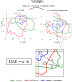
\includegraphics[width=19pc]{schematic.pdf}
\caption{Illustration of method for calculating the \textit{difference of absolute errors} (DAE) in the diurnal signal of an unedited model guidance dataset, and the human edited official forecast dataset.}
\label{Fig:schematic}
\end{figure}

The first metric I consider is the \textit{difference of absolute errors} (DAE) in the perturbations, with Fig.~\ref{Fig:schematic} illustrating how DAE is calculated. To compare errors in the diurnal signals of the official forecast and model guidance, I calculate the Euclidean distances between the official or model guidance perturbation vectors at each hour UTC, and the corresponding AWS perturbation vectors at each hour UTC, and take their difference, viewing the Euclidean distance as a measure of absolute error.

For example, to assess whether the official forecast perturbations, $\mathbf{u}_{\text{O}}$, or ACCESS perturbations, $\mathbf{u}_{\text{A}}$, produce lower absolute errors when compared with the observed AWS perturbations, $\mathbf{u}_{\text{AWS}}$, I calculate 
\begin{equation}
\text{DAE}_\text{A} = \left\lvert \mathbf{u}_{\text{AWS}}-\mathbf{u}_{\text{A}} \right\rvert - \left\lvert \mathbf{u}_{\text{AWS}}-\mathbf{u}_{\text{O}} \right\rvert. \label{Eq:DAE}
\end{equation} 
The analogously defined quantities $\text{DAE}_\text{H}$ and $\text{DAE}_\text{OCF}$ provide a comparison of the official forecast and HRES perturbations, and of the official forecast and OCF perturbations, respectively. I then calculate statistics from the DAE values on an hourly basis, in particular, I average all the 00:00 UTC DAE values, denoting such an average by $\overline{\text{DAE}}$, and repeat this for each hour of the day. If $\overline{\text{DAE}}>0$ at a particular hour, then the official forecast perturbations at that hour are on average closer to the observed perturbations than model guidance, and vice versa if $\overline{\text{DAE}}<0$.

Diurnal processes like the sea-breeze and boundary layer mixing depend on the background atmospheric conditions in which they occur. By comparing wind perturbations rather than the overall wind fields I am not claiming these background conditions are irrelevant to these processes. However, when a forecaster makes an edit of a wind forecast to better resolve these processes, they are implicitly assuming that future background conditions will be close enough to the preceding 24 hour mean state, or to model predictions of the mean state, to justify making the edit. Thus, it makes sense to compare forecast perturbations to observed perturbations, as long as differences are interpreted as a consequence not only of how the forecaster or model resolves diurnal processes, but of how differences in the background state contribute to differences in the perturbations. To minimise the importance of background state differences, this study focuses exclusively on lead-day one forecasts.

Given the large degree of turbulence or random variability in both the AWS, official, and model datasets, care must be taken to avoid pre-emptively concluding the official forecast has outperformed model guidance when $\overline{\text{DAE}}>0$ purely by chance. The method for estimating confidence in $\overline{\text{DAE}}$ is based on a method proposed by \citet{griffiths17}. Time series formed from the DAE values at a particular time, say 00:00 UTC, across the three month time period, are treated as an independent sample of a random variable $E$. The sampling distribution for each $\overline{\text{DAE}}$ can be modelled by a Student's $t$-distribution, and from this I calculate the probability that $E$ is positive, denoted $\pr\left(E > 0\right)$. 

Although temporal autocorrelations of DAE, i.e.~correlations between DAE values at a particular hour from one day to the next, are in practice small or non-existent, they are still accounted for by reducing the ``effective" sample size to $ n \left(1-\rho_1\right)/\left(1+\rho_1\right)$, where $n$ is the actual sample size and $\rho_1$ is the lag-1 autocorrelation \citep{zwiers95,wilks11}. In the language of statistical hypothesis testing, the null hypothesis that $E=0$ would be rejected at significance level $\alpha$ if $\pr(E>0) > 1-\frac{\alpha}{2}$ or $\pr(E<0) > 1-\frac{\alpha}{2}$. However, in this study I simply state the value of $\pr(E>0)$, referring to this as a \textit{confidence score}, and noting $\pr(E<0) = 1- \pr(E>0)$. I say the official forecast outperforms model guidance with ``high confidence" if $\pr(E>0) \geq 95\%$, or that model guidance outperforms the  official forecast with ``high confidence" if $\pr(E>0) \leq 5\%$, with high confidence implicit whenever it is not explicitly mentioned.

\begin{figure*}
\centering
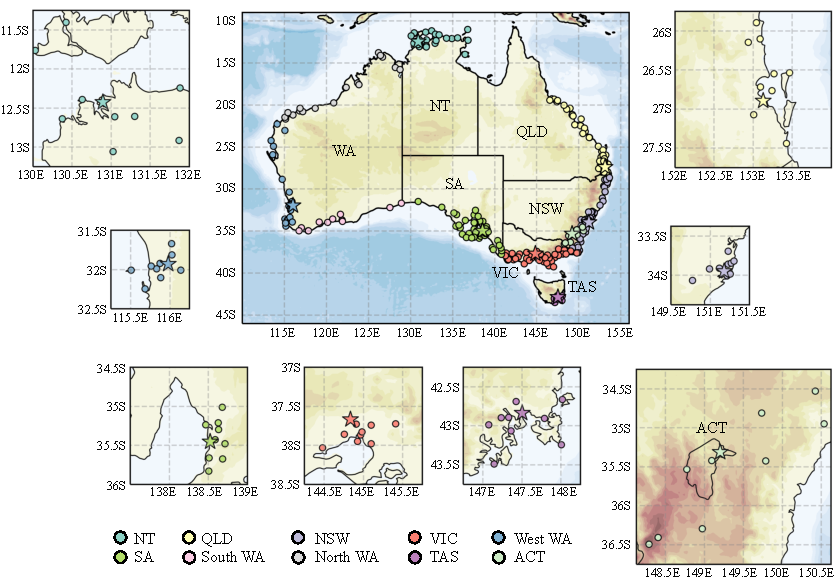
\includegraphics[width=39pc]{map.pdf}
\caption{Locations of the automatic weather stations, and the groupings of these stations, considered in this study. The \textit{coastal station groups} are indicated in a), with the \textit{airport stations} shown by stars. The Perth, Adelaide, Melbourne, Hobart, Darwin, Brisbane and Sydney \textit{city station groups} are shown shown by b) to h), respectively.}
\label{Fig:map}
\end{figure*}

Following the ``fuzzy verification" approach outlined by \citet{ebert08}, forecast and observational perturbation datasets are compared not only at individual stations, but are also averaged over two coarser spatial scales before being compared. The individual stations I consider are the 8 capital city \textit{airport stations}, marked by stars in Fig.~\ref{Fig:map}, as their high operational significance means that they are typically the most well maintained. An intermediate spatial scale is formed by averaging perturbation data over the 10 stations closest to each capital city airport station, with some flexibility allowed to ensure stations are roughly parallel to the nearest coastline. These station groups are referred to as the \textit{city station groups}. The coarsest spatial scale is formed by averaging over all stations within 150 km of the nearest coastline, and grouping these by state. The Western Australian coastline is subdivided into three pieces, and stations along the Gulf of Carpentaria, north Queensland Peninsula, and Tasmanian coastlines are neglected, in order to ensure each station group corresponds to an approximately linear segment of coastline to better resolve the land-sea breeze after spatial averaging \citep[e.g.][]{vincent16}. These eight station groups are referred to as the \textit{coastal station groups}.

To compare errors in the perturbations over the two coarser spatial scales, I modify the definition of DAE in equation (\ref{Eq:DAE}) so that each perturbation dataset is first spatially averaged over either the city or coastal station groups. Confidence scores are calculated for the city and coastal station groups in the same way as for the individual airport stations, treating the spatially averaged data as a single time series. This provides a conservative way to deal with spatial correlation between the stations in each group \citep{griffiths17}. 

To compare biases in the diurnal cycles of each dataset, I calculate the \textit{difference of biases} (DB),
\begin{equation}
\text{DB}_{\text{A}} = \left\lvert \overline{\mathbf{u}}_{\text{AWS}}-\overline{\mathbf{u}}_{\text{O}} \right\rvert - \left\lvert \overline{\mathbf{u}}_{\text{AWS}}-\overline{\mathbf{u}}_{\text{A}} \right\rvert,
\end{equation}
with $\text{DB}_{\text{H}}$ and $\text{DB}_{\text{OCF}}$ defined analogously, where the over-bars denote temporal averages of the perturbations at a particular hour, over June, July and August 2018. These temporally averaged perturbations can be viewed as the mean diurnal wind cycles over the three month study period for each dataset. Biases over the city and coastal station groups are calculated by taking the spatial average before the temporal average. Uncertainty in the DB is estimated through bootstrapping \citep{efron79}. This is done by performing resampling with replacement on the underlying perturbation datasets, and calculating the DB 1000 times using these resampled datasets. This provides a distribution of DB values, which analogously to with DAE, I treat as a sample from a random variable $B$, and use this to estimate $\pr\left(B > 0\right)$.

Note that on a given day, at a given location, wind perturbations do not necessarily reflect genuinely diurnal processes. There is a large degree of random turbulence in AWS wind observations, and convective cold pools or synoptic fronts can produce rapid changes in winds that induce large perturbations. However, by averaging multiple perturbations at a given hour over many days, I cancel as much of this non-diurnal variability as possible. When this is repeated for each hour of the day, the signal that remains reflects the mean diurnal cycle (e.g. Figs.~\ref{Fig:darwin_hodo} and \ref{Fig:clim_hodo}). Similar ideas apply to the DAE metric, but because perturbations are compared before temporal averaging, then the DAE itself temporally averaged, $\overline{\text{DAE}}$ is more sensitive to random variability than DB, and measures of confidence become particularly important. Note that spatially averaging perturbations accomplishes a similar thing to temporal averaging, helping to cancel out random variability. These ideas can be explored with synthetic data, and some preliminary work to this end is available online \citep{short20}.

Another approach to forecast verification is to assess structural features of the phenomena being forecast rather than errors or biases of point predictions; this approach is particularly important at small spatiotemporal scales \citep[e.g.][]{mass02, rife05}. \citet{gille05} obtained summary statistics on the observed structure of mean diurnal wind cycles by using linear regression to calculate the coefficients $u_i$, $v_i$ $i=0,1,2$, for the fits 
\begin{align}
u &= u_0 + u_1 \cos(\omega t) + u_2 \sin(\omega t), \label{Eq:u_h} \\
v &= v_0 + v_1 \sin(\omega t) + v_2 \sin(\omega t), \label{Eq:v_h}
\end{align}
where $\omega$ is the angular frequency of the earth and $t$ is the local solar time in seconds. These fits trace out ellipses in the $x,y$ plane, and descriptive metrics like the eccentricity of the ellipse and the angle the semi-major axis makes with lines of latitude, can be calculated directly from the coefficients $u_1$, $u_2$, $v_1$ and $v_2$. \citet{gille05} applied this fit to scatterometer data, which after temporal averaging resulted in just four zonal and meridional values per location, and as such the fit performed very well.  

However, equations (\ref{Eq:u_h}) and (\ref{Eq:v_h}) do not provide a good fit for the hourly data considered here, primarily because they assume a twelve hour symmetry in the evolution of the diurnal cycle. In practice, asymmetries between daytime heating and nighttime cooling \citep[e.g.][]{svensson11} result in surface wind perturbations accelerating rapidly just after sunrise, but remaining comparatively stagnant at night (e.g.~Fig.~\ref{Fig:clim_hodo}). Thus, I instead fit the equations
\begin{align}
u &= u_0 + u_1 \cos(\alpha(\psi,t)) + u_2 \sin(\alpha(\psi,t)), \label{Eq:u} \\
v &= v_0 + v_1 \sin(\alpha(\psi,t)) + v_2 \sin(\alpha(\psi,t)), \label{Eq:v}
\end{align}
to the climatological perturbations, with $\alpha$ the function from $[0,24) \times [0, 2\pi) \to [0, 2\pi)$ given by
\begin{equation}
\alpha(\psi,t) \equiv \pi \left[\sin\left( \pi \frac{(t - \psi)  \bmod 24}{24} - \frac{\pi}{2} \right) + 1 \right], \label{Eq:alpha}
\end{equation}
with $t$ the time in units of hours UTC, and $\psi$ providing the time when the wind perturbations vary least with time, noting that the same value of $\psi$ is used for both the zonal and meridional perturbations. For each climatological diurnal wind cycle, I solve for the seven parameters $u_0$, $u_1$, $u_2$, $v_0$, $v_1$, $v_2$ and $\psi$ using non-linear regression.

Importantly, the metrics defined in this section compare just \textit{some aspects} of the official forecast with model guidance: they do not, for instance, assess whether diurnal variance of the official forecast is more realistic than that of model guidance. Thus, any statements about performance made throughout this paper refer solely to the metrics defined here, and \textit{no claim} is being made that these are sufficient to completely characterise the accuracy, or value to the user, of how the diurnal wind cycle is represented in competing forecasts.

\section{Results}
\label{Sec:Results}
In this section, the methods described in section \ref{Sec:Methods} are applied to Australian forecast and station data over the months of June, July and August 2018. First, mean differences in absolute errors (DAE) and differences in biases (DB) over this time period are assessed. Second, structural indices are compared to elucidate the physical reasons for biases. Unless otherwise noted, times are given in UTC.

\begin{figure*}
\centering
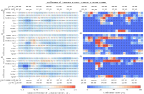
\includegraphics[width=39pc]{wpi_coastal_new_colours.pdf}
\caption{Heatmaps of mean difference of absolute error $\overline{\text{DAE}}$ values, a), c), e), and confidence scores, b), d), f), for each coastal station group (see Fig.~\ref{Fig:map}) and hour of the day, for the official forecast versus ACCESS, a) and b), official forecast versus HRES, c) and d), and official forecast versus OCF, e) and f), comparisons. Positive $\overline{\text{DAE}}$ values indicate that the former dataset in each pair is on average $\overline{\text{DAE}}$ kn closer to observations than the latter dataset (see equation \ref{Eq:DAE}), where $1$ kn $\approx 0.514$ m s\textsuperscript{-1}. Confidence scores provide the probability the population or ``true" value of $\overline{\text{DAE}}$ is greater than zero (see section \ref{Sec:Methods}).}
\label{Fig:wpi_coastal}
\end{figure*}

\begin{figure}
\centering
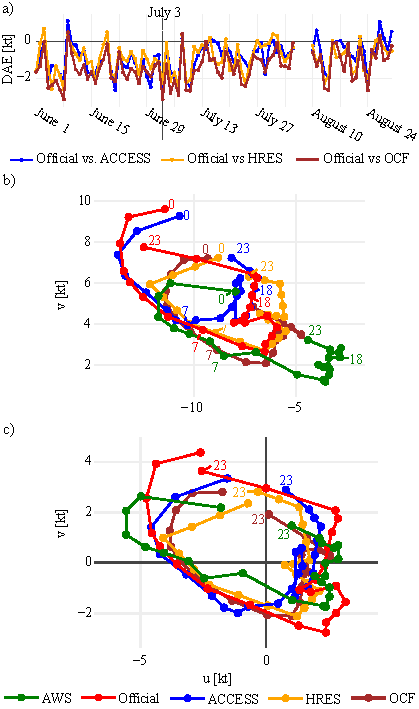
\includegraphics[width=19pc]{case_studies_nt.pdf}
\caption{Time series, a), of the difference in absolute error DAE defined in equation (\ref{Eq:DAE}) for the official forecast versus ACCESS, $\text{DAE}_\text{A}$, official forecast versus HRES, $\text{DAE}_\text{H}$, and official forecast versus OCF, $\text{DAE}_\text{OCF}$ comparisons, for the Northern Territory (NT) coastal station group shown in Fig.~\ref{Fig:map} at 23:00 UTC. Also, temporal hodographs in hours UTC showing hourly changes in winds, b), and wind perturbations from a 24 hour running mean, c), at the NT coastal station group on the 3\textsuperscript{rd} of July 2018.}
\label{Fig:case_studies_nt}
\end{figure}

\subsection{Absolute Errors}
\label{Sec:Daily}

Figure \ref{Fig:wpi_coastal} provides the mean difference of absolute error values and confidence scores defined in section \ref{Sec:Methods} for the coastal station groups shown in Fig.~\ref{Fig:map}. Results are given for the official forecast versus ACCESS, official forecast versus HRES, and official forecast versus OCF comparisons, denoted by $\overline{\text{DAE}}_\text{A}$, $\overline{\text{DAE}}_\text{H}$ and $\overline{\text{DAE}}_\text{OCF}$, respectively. The results indicate that for the majority of station groups and hours, the unedited ACCESS, HRES and OCF datasets outperform the official forecast. The lowest $\overline{\text{DAE}}$ values occur at the Northern Territory (NT) station group at 23:00 and 00:00 for both $\overline{\text{DAE}}_\text{A}$ and $\overline{\text{DAE}}_\text{H}$, and at 22:00 and 23:00 for $\overline{\text{DAE}}_\text{OCF}$. Although the official forecast outperforms at least one of ACCESS, HRES and OCF at multiple times and station groups, the only group and time where it outperforms all three is 05:00 UTC over the South WA station group.

Figures \ref{Fig:case_studies_nt} and \ref{Fig:case_studies_wa} provide case studies of the NT and South Western Australia (WA) station groups, respectively. Figure \ref{Fig:case_studies_nt} a) provides a time series of DAE for the NT station group at 23:00. The time series shows significant temporal variability, with DAE frequently dropping below $-2$ kn. Figures \ref{Fig:case_studies_nt} b) and c) show hodographs of the winds and wind perturbations, respectively, at each hour UTC on the 3\textsuperscript{rd} of July, which provides an interesting example. 

Figure \ref{Fig:case_studies_nt} b) shows that the official wind forecast on this day was likely based on edited ACCESS from 00:00 to 06:00, then edited HRES from 07:00 to 13:00 UTC, then unedited ACCESS from 15:00 to 21:00. At 22:00 and 23:00, the official forecast winds acquire stronger east-southeasterly components than the other datasets. For comparison, Fig.~\ref{Fig:perth_sounding} a) shows the first ten values from wind soundings at Darwin Airport at 12:00 on July 3\textsuperscript{rd} and 00:00 on July 4\textsuperscript{th}. In both instances the winds are east-southeasterly, and so the rapidly changing wind perturbations at 22:00 in the official forecast may reflect a boundary layer mixing edit that has been applied either too early, or has strengthened the southeasterly component of the winds too much. Similar issues appear to create the low DAE values on the 8\textsuperscript{th} of June and 9\textsuperscript{th} and 10\textsuperscript{th} of July.

Figure \ref{Fig:case_studies_wa} a) provides a time series of DAE for the South WA station group at 05:00. As with the NT station group there is significant temporal variability, with DAE frequently exceeding 1 kn. Figures \ref{Fig:case_studies_wa} b) and c) provide hodographs of the winds and wind perturbations, respectively, on the 9\textsuperscript{th} of June, another interesting example. Both the raw winds and the perturbations appear to show both HRES and ACCESS under-predicting the amplitude of the diurnal wind cycle on this day, with OCF performing better in this regard. Figure \ref{Fig:perth_sounding} b) shows wind soundings at Perth Airport, the nearest station to provide wind soundings, between 12:00 on the 8\textsuperscript{th} June and 12:00 on the 9\textsuperscript{th} June. The 8\textsuperscript{th} June 12:00 sounding shows surface northerlies of around $6$ kn, becoming west to northwesterlies of over 20 kn $2.4$ km above the surface. However, the subsequent sounding at 00:00 on the 9\textsuperscript{th} of June shows that the winds acquire a strong northerly component of 30 kn in the first 500 m of the atmosphere, with the final sounding indicating a strong northwesterly wind at 725 m persisting until 12:00. 

In Fig.~\ref{Fig:case_studies_wa} c), the OCF and official forecast perturbations from 04:00 to 07:00 show stronger westerly perturbations than either ACCESS or HRES, improving the magnitude of both dataset's perturbations. However, the AWS perturbations are more northerly than those of the official forecast or OCF. Possible explanations for this discrepancy are that the official forecast has been edited based on the June 8\textsuperscript{th} 12:00 UTC sounding, with the winds above the surface changing direction in the subsequent 12 hours, or that the official forecast has been based on OCF, which underestimates the northerly component of the perturbations.

\begin{figure}
\centering
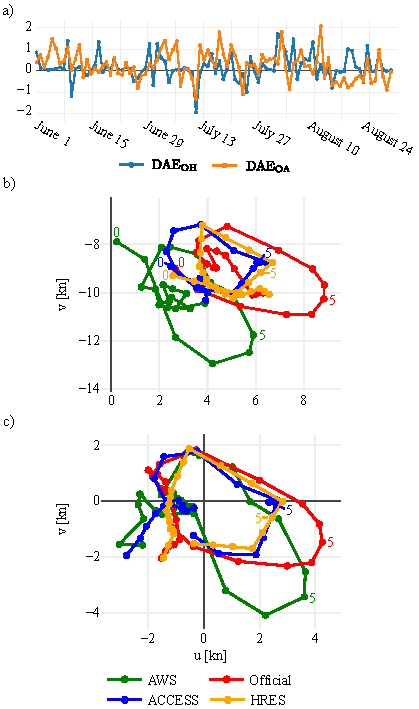
\includegraphics[width=19pc]{case_studies_wa.pdf}
\caption{As in Fig.~\ref{Fig:case_studies_nt}, but for, a), the South WA coastal station group at 05:00 UTC, and b) and c), the winds and wind perturbations, respectively, over the South WA coastal station group on the 9\textsuperscript{th} June 2018.} 
\label{Fig:case_studies_wa}
\end{figure}

\begin{figure*}
\centering
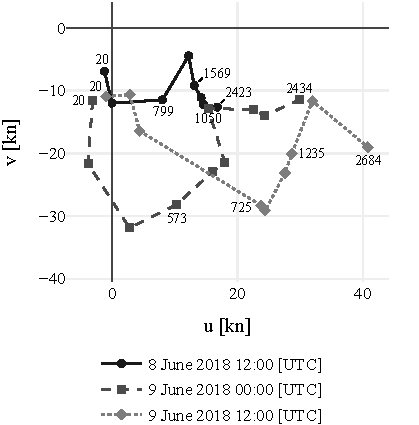
\includegraphics[width=33pc]{perth_sounding.pdf}
\caption{Vertical wind soundings at, a), Darwin Airport, and b), Perth Airport, with heights given in metres.}
\label{Fig:perth_sounding}
\end{figure*}

\begin{figure*}
\centering
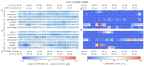
\includegraphics[width=39pc]{airport_wpi_new_city.pdf}
\caption{As in Fig.~\ref{Fig:wpi_coastal}, but for the official versus HRES mean difference of absolute error $\overline{\text{DAE}}_\text{OH}$ values, a) and c), and confidence scores, b) and d), for the airport stations, a) and b), and city station groups, c) and d).}
\label{Fig:city_wpi}
\end{figure*}

\begin{figure*}
\centering
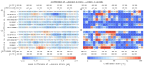
\includegraphics[width=39pc]{airport_wpi_new_airports.pdf}
\caption{As in Fig.~\ref{Fig:wpi_coastal}, but for the official versus HRES mean difference of absolute error $\overline{\text{DAE}}_\text{OH}$ values, a) and c), and confidence scores, b) and d), for the airport stations, a) and b), and city station groups, c) and d).}
\label{Fig:airport_wpi}
\end{figure*}

Fig.~\ref{Fig:city_wpi} presents the $\overline{\text{DAE}}$ values and confidence scores for the city station groups, for the official forecast versus HRES and official forecast versus OCF comparisons; the official forecast versus ACCESS comparisons (not shown) are similar to those for HRES and have been omitted for space. Both HRES and OCF outperform the official forecast almost uniformly, with the Darwin city station group the main exception. At Darwin, the official forecast outperforms HRES at 02:00 UTC, and there is ambiguity as to whether the official forecast or HRES performs better at some other times of day. The OCF comparison shows less ambiguity at Darwin, but more at Melbourne and Brisbane. The city station group results for December, January, February 2017/18 (not shown) are similar but slightly more ambiguous, particularly for ACCESS.  

Fig.~\ref{Fig:airport_wpi} presents the comparisons for the airport stations. Here the results are noisier than at both the city and coastal spatial scales, but similarities also exist. For instance, the official forecast outperforms both OCF and HRES at 02:00 UTC at Darwin airport, the Darwin city station group, and the NT coastal station group with at least $90\%$ confidence. There are four other instances where the official forecast outperforms HRES with at least $90\%$ confidence, although this could simply be occurring by chance due repeated testing \citep[p. 178]{wilks11}. By contrast, the official forecast outperforms OCF over four hour intervals at both Perth and Brisbane airports.

\subsection{Seasonal Biases}
\label{Sec:Seasonal}
Figure \ref{Fig:cwpi_coastal} provides the difference of biases (DB) and confidence scores defined in section \ref{Sec:Methods}, for the coastal station groups, for the official forecast versus ACCESS, official forecast versus HRES, and official forecast versus OCF comparisons. At the NT station group at 03:00, the official forecast outperforms both ACCESS and HRES with confidence $\geq 93\%$. However, ACCESS, HRES and OCF each outperform the official forecast at 23:00 and 00:00, and from 06:00 to 10:00, consistent with the $\overline{\text{DAE}}$ results of Fig.~\ref{Fig:wpi_coastal}. Figure \ref{Fig:darwin_hodo} c) shows that these DB results reflect amplitude biases in the official forecast's diurnal cycle.

\begin{figure*}
\centering
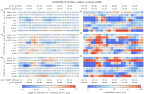
\includegraphics[width=39pc]{cwpi_coastal_reformed.pdf}
\caption{As in Fig.~\ref{Fig:wpi_coastal}, but for the difference of biases (DB) values and confidence scores.}
\label{Fig:cwpi_coastal}
\end{figure*}

\begin{figure*}
\centering
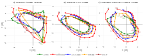
\includegraphics[width=39pc]{darwin_hodo.pdf}
\caption{Temporal hodographs in hours UTC of wind perturbations at, a), Darwin Airport, and b), spatially averaged over the Darwin city station group, and c), the NT coastal group (see Fig.~\ref{Fig:map}), then temporally averaged over June, July and August 2018.}
\label{Fig:darwin_hodo}
\end{figure*}

At the South WA station group from 01:00 to 05:00 UTC, the official forecast outperforms HRES with confidence scores of at least $88\%$. Figure \ref{Fig:clim_hodo} a) shows that HRES underestimates the westerly perturbations at these times, with these perturbations potentially associated with boundary layer mixing processes, as discussed in section \ref{Sec:Results} \ref{Sec:Daily}. The official forecast, ACCESS and HRES all underestimate the amplitude of the diurnal cycle between 02:00 and 10:00, including both the westerly perturbations and the southerly sea-breeze perturbations. OCF better approximates the amplitude of the diurnal cycle between 02:00 and 05:00, but shows the greatest underestimation of the southerly perturbations between 06:00 and 10:00.

At the South Australia (SA) station group, the official forecast slightly outperforms ACCESS and HRES from 02:00 to 05:00 and 09:00 to 12:00, although confidence scores do not exceed 88\% and 65\% respectively. The official forecast also slightly outperforms OCF between 00:00 and 02:00, and between 08:00 and 09:00, although confidence scores do not exceed 75\%. Figure \ref{Fig:clim_hodo} b) shows that although the official forecast captures the amplitude of the perturbations from 01:00 to 05:00 UTC almost perfectly, its diurnal cycle is out of phase with that of the AWS during this period, explaining the only slightly positive DB values.

\begin{figure}
\centering
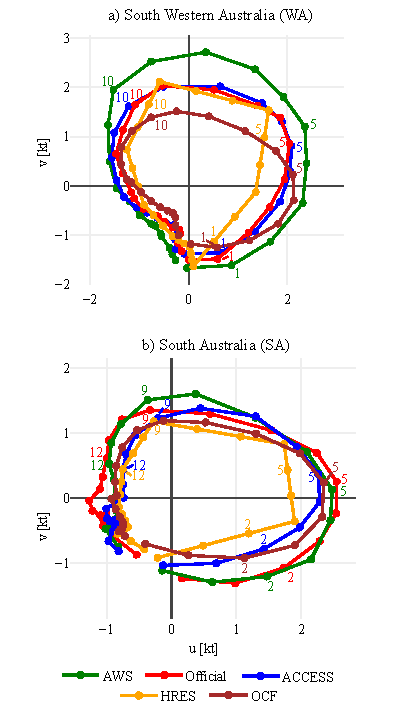
\includegraphics[width=19pc]{clim_hodo_alt.pdf}
\caption{Temporal hodographs in hours UTC of wind perturbations spatially averaged over the, a), South Western Australia (WA), and b), South Australia (SA) coastal station groups (see Fig.~\ref{Fig:map}), and temporally averaged over June, July and August 2018.}
\label{Fig:clim_hodo}
\end{figure}

For comparison, Figs.~\ref{Fig:cwpi_city} and \ref{Fig:cwpi_airport} present the DB values and confidence scores for the official forecast versus HRES and official forecast versus OCF comparisons, for the city station groups and airport stations, respectively. Some regions exhibit consistent results across all three spatial scales. For example, the official forecast diurnal signal is less biased than HRES between 14:00 and 18:00, with at least $85\%$ confidence, at Sydney airport, the Sydney city station group, and the NSW coastal station group. 

Other results are markedly different between spatial scales. For instance, the official forecast outperforms OCF for most of the day at Darwin airport, but the opposite is true at the Darwin city and NT coastal station groups. Figure \ref{Fig:darwin_hodo} a) shows that the mean AWS diurnal cycle is highly asymmetric, with a sharp peak occurring at 06:00. This peak is captured well by HRES and the official forecast, but not by OCF or ACCESS. Figures \ref{Fig:darwin_hodo} b) and c) show that over the Darwin city and NT coastal station groups, the diurnal cycles are much smoother, with the amplitudes of the official forecast diurnal cycles exaggerated relative to AWS and OCF. 

\begin{figure*}
\centering
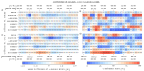
\includegraphics[width=39pc]{cwpi_city.pdf}
\caption{As in Fig.~\ref{Fig:airport_wpi}, but for the difference of biases (DB) values and confidence scores.}
\label{Fig:cwpi_city}
\end{figure*}

\begin{figure*}
\centering
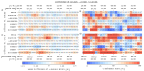
\includegraphics[width=39pc]{cwpi_airport.pdf}
\caption{As in Fig.~\ref{Fig:airport_wpi}, but for the difference of biases (DB) values and confidence scores.}
\label{Fig:cwpi_airport}
\end{figure*}

\subsection{Ellipse Fits}

\begin{figure}
\centering
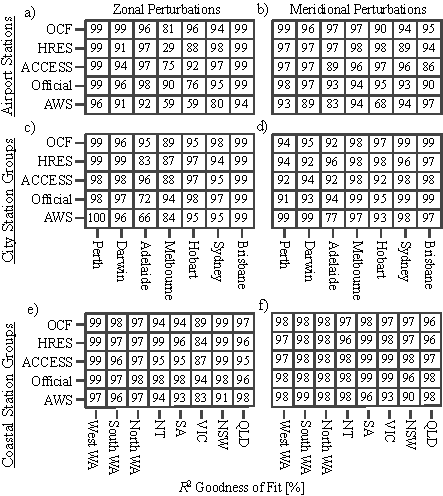
\includegraphics[width=19pc]{r_squared.pdf}
\caption{$R^2$ values as percentages for the fit of equation (\ref{Eq:u}) to the zonal perturbations, a), c) and e), and equation (\ref{Eq:v}) to the meridional perturbations, b), d) and f), for the airport stations, a) and b), city station groups, c) and d), and coastal station groups, e) and f), shown in Fig.~\ref{Fig:map}.}
\label{Fig:r_squared}
\end{figure}

The hodographs in Figs.~\ref{Fig:darwin_hodo} and \ref{Fig:clim_hodo} are roughly elliptical in shape, suggesting that descriptive quantities can be estimated by fitting equations (\ref{Eq:u}) and (\ref{Eq:v}) to the zonal and meridional mean perturbations, as described in section \ref{Sec:Methods}. Figure \ref{Fig:r_squared} gives the $R^2$ values for the fits of the zonal and meridional perturbations to equations (\ref{Eq:u}) and (\ref{Eq:v}), respectively. The fit performs best at the coastal station group spatial scale, with $R^2$ generally above $95\%$. 

\begin{figure*}
\centering
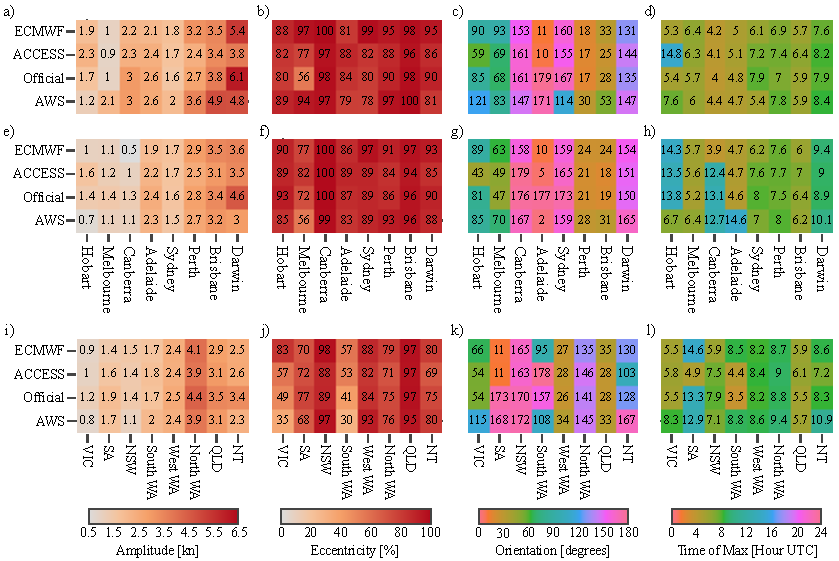
\includegraphics[width=39pc]{ellipse_fits.pdf}
\caption{Metrics derived from fitting ellipse equations (\ref{Eq:u}) and (\ref{Eq:v}) to wind perturbations at the Australian capital city airport stations, a) to d), and to wind perturbations spatially averaged over the city station groups and coastal station groups shown in Fig.~\ref{Fig:map}, e) to h) and i) to l) respectively, with perturbations also temporally averaged over June, July and August 2018 in each case. Metrics given are the maximum perturbation speed, a), e) and i), eccentricity of fitted ellipse, b), f) and j), orientation semi-major axis makes with lines of latitude, c), g) and k), and time of maximum perturbation, d), h) and l).}
\label{Fig:ellipse_fits}
\end{figure*}

Figure \ref{Fig:ellipse_fits} provides four descriptive quantities based on the fits of equations (\ref{Eq:u}) and (\ref{Eq:v}) to the mean perturbations: these are maximum perturbation speed, eccentricity of the fitted ellipse, angle the semi-major axis makes with lines of latitude, and the time at which the maximum perturbation speed is achieved. 

Figure \ref{Fig:ellipse_fits} a) indicates OCF has significant mean diurnal cycle amplitude biases at the airport station scale, with the exception of Hobart. These biases persist, but are smaller, at the city station group scale, but are absent at the coastal station group scale, with the exception of  Queensland (QLD). Given that OCF represents a blended average of multiple model guidance datasets \citep{engel07}, and that OCF's gridding process involves additional interpolation steps \citep{bom08, bom12}, this result is not surprising: at the individual station scale OCF has undergone more smoothing than ACCESS or HRES, but at the coarser spatial scales this lessens in importance as all datasets undergo comparable smoothing. Note that this does \textit{not} mean OCF's overall wind speeds or directions are biased at the individual station scale, only the amplitude of OCF's mean diurnal cycle, \textit{as it has been defined} in this study. 

Considering specific locations, Brisbane provides an interesting example, as Fig.~\ref{Fig:ellipse_fits} a) shows that at Brisbane airport the maximum AWS perturbation is at least $1$ kn greater than the official forecast, ACCESS and HRES, and $3.5$ kn greater than that of OCF. Furthermore Fig.~\ref{Fig:ellipse_fits} c) shows that the orientation of the AWS fitted ellipse is at least 20 degrees anti-clockwise from that of the other datasets. 

Figures \ref{Fig:ellipse_hodo} a) and b) show hodographs of the Brisbane airport mean perturbations and ellipse fits, respectively. Although the ellipse fits suppress some of the asymmetric details, they capture the amplitudes and orientations of the real mean diurnal cycles well. In this case the results show that the average AWS sea-breeze approaches from the northeast, whereas the official forecast, HRES, ACCESS and OCF sea-breezes approach more from the east-northeast. The amplitude of OCF's diurnal cycle is significantly weaker than those of the other datasets.  

To check whether these results just represent a direction bias of the Brisbane Airport weather station, Fig.~\ref{Fig:ellipse_hodo} c) shows the mean perturbations at the nearby Spitfire Channel station (see Fig.~\ref{Fig:map}). While the amplitude biases are slightly smaller at Spitfire Channel than Brisbane Airport, the directional bias is at least as high. A similar directional bias is evident at the nearby Inner Beacon station (not shown), although the bias is smaller than at Spitfire Channel and Brisbane Airport. Similar biases are also evident at these stations in analogous figures for December, January and February 2017/18 (not shown), with the semi-major axis of the official forecast's ellipse fit oriented $29^\circ$ clockwise from AWS's at Brisbane airport. Figure \ref{Fig:map} shows there are two small islands to the east of Brisbane airport; the more north-northeasterly orientation of the Brisbane Airport sea-breeze suggests these islands may be redirecting winds between the east coast of Brisbane and the west coasts of these islands, and that this local effect is not being captured in the official forecast, ACCESS, HRES or OCF.  

\begin{figure*}
\centering
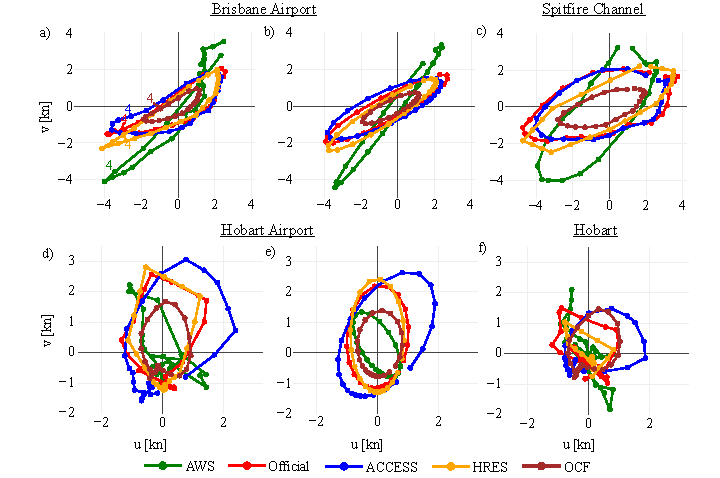
\includegraphics[width=39pc]{ellipse_hodo.pdf}
\caption{Temporal hodograph, a), and ellipse fit, b), of wind perturbations at each hour UTC averaged over June, July and August 2018 at Brisbane airport. For comparison, c) provides the hodograph of the mean perturbations at the nearby Spitfire Channel station (see Fig.~\ref{Fig:map}).}
\label{Fig:ellipse_hodo}
\end{figure*}

The South WA station group provides another interesting example, as Fig.~\ref{Fig:ellipse_fits} shows the semi-major axes of the ACCESS and official forecast ellipse fits are oriented at least 48 degrees anti-clockwise from those of the AWS and HRES ellipse fits, and the HRES perturbations peak between 1.2 and 4 hours after the other datasets. Figure \ref{Fig:clim_hodo} a) shows that these differences occur because the westerly perturbations, likely associated with boundary layer mixing, are weaker for HRES than for the other datasets. A similar issue affects the Victorian (VIC) station group, explaining why the semi-major axes of the AWS ellipse fit is oriented at least 49 degrees anti-clockwise from those of HRES, ACCESS and the official forecast. 

The Darwin Airport, Darwin Airport station group, and NT station group (not shown) provide further examples. Here the ellipse fits slightly underestimate the AWS maximum perturbation speed at Darwin Airport due to this dataset's highly asymmetric hodograph. At all three spatial scales there are timing differences between the perturbation maximums of up to 8.2 hours. These timing differences occur because for some scales and datasets, the later north to northwesterly sea-breeze perturbations dominate the mean diurnal wind cycle, but for other scales and datasets the earlier easterly to southeasterly boundary layer mixing perturbations dominate.

\section{Synthesis}
\label{Sec:Discussion}
For land-sea breeze and boundary layer mixing edits to reduce absolute errors in the subsequent days wind forecast, these edits should reduce the absolute errors in the diurnal component of the wind fields. However, Figs.~\ref{Fig:wpi_coastal},\ref{Fig:airport_wpi} indicate that this is generally only possible when absolute error is considered at coarse spatial scales, as at individual airport stations results are generally noisy and ambiguous, and over the intermediate city station group scale HRES and OCF outperform the official forecast almost uniformly.

Taking the effective resolutions of the models considered in this study to be approximately $7\Delta x$ \citep[e.g.][]{skamarock04, abdalla13}, where $\Delta x$ is the horizontal grid spacing, the effective resolutions of ACCESS and HRES are $\approx 84$ km and $\approx 63$ km, respectively. From resolution considerations alone, one might expect that forecaster edits would be able to reduce errors at the individual airport station scale, and the intermediate city station group scale (see Fig.~\ref{Fig:map}), as motion at these scales is unresolved or only partially resolved by ACCESS and HRES.

To further investigate the effect of spatial scale on error, consider first just the zonal components of the AWS and official forecast wind perturbations, denoted by $u_\text{AWS}$ and $u_\text{O}$ respectively. Considering just the values at a particular hour UTC, over the entire June, July, August time period, the mean square error $\mse\left(u_\text{AWS}, u_\text{O}\right) = \overline{\left(u_\text{AWS} - u_\text{O}\right)^2}$ can be decomposed $\mse\left(u_\text{AWS}, u_\text{O}\right)=$ 
\begin{equation}
\underbrace{\var\left(u_\text{AWS}\right) + \var\left(u_\text{O}\right) - 2\cov\left(u_\text{AWS}, u_\text{O}\right)}_\text{error variance} + \underbrace{\left(\overline{u}_\text{AWS} - \overline{u}_\text{O}\right)^2}_{\text{squared bias}} \label{Eq:MSE}
\end{equation}
where $\var$, $\cov$ and the over-bar denote the sample variance, covariance and mean respectively. The first three terms are the variance of $u_\text{AWS} - u_\text{O}$, i.e. the error variance, and the last term is the square of the bias between $u_\text{AWS}$ and $u_\text{O}$. Equation (\ref{Eq:MSE}) can also be applied to the mean square errors (MSEs) of ACCESS, HRES and OCF. Note that the MSE is closely related to $\overline{\text{DAE}}$, which is the difference between the mean absolute errors of the official forecast and HRES; similarly, the squared bias components of the MSEs are closely related to $\text{DB}$. 

\begin{figure*}
\centering
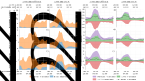
\includegraphics[width=39pc]{error_decomp_bris.pdf}
\caption{Mean square error between the AWS and HRES zonal perturbations $\overline{\left(u_\text{AWS} - u_\text{H}\right)^2}$, a), e), and i), decomposed into the error variance $\var\left(u_\text{AWS} - u_\text{H}\right)$ and squared bias $\left(\overline{u}_\text{AWS} - \overline{u}_\text{H}\right)^2$ terms of equation (\ref{Eq:MSE}). Also, the decomposed mean square error between the AWS and official forecast zonal perturbations, b), f) and j). Additionally, the HRES and AWS error variance term $\var\left(u_\text{AWS} - u_\text{H}\right)$ decomposed into the $\var\left(u_\text{AWS}\right)$, $\var\left(u_\text{H}\right)$ and  $- 2 \cdot \cov\left(u_\text{AWS}, u_\text{H}\right)$ terms, c), g) and k), and analogously for the official forecast and AWS error variance term $\var\left(u_\text{AWS} - u_\text{O}\right)$, d), h) and l). Decompositions given for Brisbane Airport, a) to d), the Brisbane city station group, e) to h), and the Queensland coastal station group, i) to l). See Fig.~\ref{Fig:map} for station locations.}
\label{Fig:error_decomp_bris}
\end{figure*}

Figure \ref{Fig:error_decomp_bris} shows the terms of equation (\ref{Eq:MSE}) for both the official forecast and OCF for Brisbane Airport, the Brisbane city station group, and the QLD coastal station group. At all three scales the official forecast varies more than OCF. The official forecast also generally varies more than ACCESS and HRES (not shown), and this is also true for the other stations and station groups considered in this study. 

At Brisbane airport the variance of AWS is significantly larger than either the official forecast or OCF. This additional variability is mostly uncorrelated to either dataset; although the covariance between the official forecast and AWS increases between 20:00 and 08:00, the increase is not sufficient to offset the official forecast's additional variance, and the error variances are thus of comparable magnitude for both the official forecast and OCF. 

The larger AWS variances are unsurprising from representation considerations alone \citep[e.g.][]{zaron06}, as the official forecast and OCF data represent averages over 6 km spatial grid-cells, whereas the AWS data represent point values. As a result, error variance terms are generally much larger than the squared bias terms at this scale. The exception is OCF at 04:00, where the squared bias is $\approx 6$ kn, while error variance is $\approx 15$ kn. This results in a higher MSE for OCF than the official forecast around 04:00, consistent with the airport station $\overline{\text{DAE}}$ results of Fig.~\ref{Fig:airport_wpi} c) and d).

At the intermediate Brisbane city station group scale, the AWS variances are again larger than those OCF, but of comparable magnitude to those of the official forecast, with the official forecast's additional variability again mostly uncorrelated to AWS. This results in larger error variance terms for the official forecast, consistent with OCFs almost complete outperformance of the official forecast in Figs.~\ref{Fig:airport_wpi} c) and d). However, OCF's bias squared terms remain larger than the official forecast's, resulting in OCF's MSE slightly exceeding the official forecast's at around 04:00. These results are consistent with Figs.\ref{Fig:city_wpi} c) and d), where the official forecast slightly outperforms OCF at 04:00 with a confidence score of $79\%$.  

Over the coarse QLD coastal station group scale, variances in all three datasets are small enough that the error variance terms are less dominant over the bias terms. Although the error variance of the official forecast is still larger than that of OCF, OCF's zonal biases around 04:00 UTC are again sufficient to result in larger MSEs around this time. When considered with the analogous plots for the meridional perturbations (not shown), for which OCFs bias squared terms peak slightly later, the results are consistent with the Figs.~\ref{Fig:wpi_coastal} c) and d). 

Analogous points can be made for the other locations and datasets considered in this study. At the airport station scale, AWS variance is generally significantly higher than that of the official forecast and model guidance, producing high error variance and  likely explaining why the airport station DAE results of Fig.~\ref{Fig:airport_wpi} are comparatively noisier than those of the city or coastal station group scales. Interesting exceptions include OCF at Brisbane and Perth airports, where amplitude biases in OCF's diurnal cycle are sufficient to affect airport station DAE scores.

At the city station group scale, the official forecast is generally outperformed by HRES and OCF in the $\overline{\text{DAE}}$ results of Fig.~\ref{Fig:city_wpi}, and in the analogous comparisons with ACCESS (not shown). This occurs because the official forecast is generally more variable than model guidance, and this additional variability is mostly random, in the sense of being uncorrelated with AWS. At the coastal station group scale, random variability in each dataset is reduced, and biases are sufficiently large relative to error variance to affect the $\overline{\text{DAE}}$ results of Fig.~\ref{Fig:wpi_coastal}.

These results show that switching model guidance products or performing edits can add more random noise to the diurnal component of the official forecast than what can be offset by reductions in bias, or improved correlations with AWS. Because the official forecast is built from multiple model datasets, switching between datasets with different means will tend to produce greater variance than any of the component datasets. If the choice of model guidance is made primarily on which model best captures more slowly evolving, larger amplitude synoptic scale features, then switching model guidance may add random variability to the diurnal component of the official forecast. Furthermore, unless all forecasters follow identical thought processes when making edits, the edits will also add random variability. 

These results could have implications for forecasting practice. Model guidance products are indeed biased in how they resolve diurnal wind cycles (e.g. Fig.~\ref{Fig:ellipse_hodo}), and there is therefore scope for forecaster edits to reduce these biases. However, editing model guidance generally fails to reduce error in the forecast diurnal cycle, even at scales finer than the effective resolutions of the models, as at these scales the cycle itself is mostly hidden by random variability. Averaging over large areas reduces this random variability, better revealing the diurnal cycle, and so biases have a greater impact on forecast error. However, even at large scales Fig.~\ref{Fig:wpi_coastal} shows model guidance still outperforms the official forecast more often than not.

Reducing the random variability of the official forecast, or the model guidance datasets that comprise it, could therefore improve the capacity of these types of edits to reduce error in the diurnal cycle. One way to accomplish this would be to use an ensemble average model guidance product like OCF, another would be to further post process model guidance products, such as by averaging multiple time steps around the hour, before including them in the GFE.

\section{Conclusion}
\label{Sec:Conclusion}
In this study I have presented methods for verifying the diurnal component of wind forecasts, with the intended application being the assessment of the edits Australian forecasters make to model guidance datasets to better resolve land-sea breeze and boundary layer mixing processes. I considered both errors and seasonal biases at each hour UTC, over three spatial scales, but the methods are immediately generalisable to other spatiotemporal scales. 

When the methods are applied to Australian forecast data, the results indicate that the official edited forecast only produces lower absolute errors in the diurnal wind cycle when averaged over coarse spatial scales of $500\times 100$ km$^{2}$ to $2000 \times 100$ km$^{2}$: this scale corresponds to the aggregation of data within 100 km of the Australian coastline, subdivided into linear segments of coastline and by state (see Fig.~\ref{Fig:map}). Even at these scales, reductions in error are isolated to particular locations and times of day, and the official forecast rarely has lower mean absolute error than the three model guidance products considered in this study simultaneously.

By contrast, the official forecast can produce lower seasonal biases than model guidance at all three spatial scales, but again, it rarely produces lower biases than the three model guidance considered here simultaneously. Reduced seasonal biases do not translate into reduced errors at the two smaller spatial scales because the diurnal cycle is mostly masked by the random variability in each dataset. Furthermore, because the official forecast generally exhibits much greater random variability than model guidance, model guidance almost uniformly outperforms the official forecast over the intermediate $50\times 50$ km$^{2}$ to $200 \times 200$ km$^{2}$ city station group spatial scale. The same is true for ACCESS, although to a slightly lesser extent.

I also compare structural features of the mean diurnal wind cycles of each dataset by fitting modified ellipses to their temporal hodographs, then deriving metrics from these ellipses. This approach reveals structural biases in the official forecast, including directional biases in the approach of the sea-breeze at Brisbane airport, and amplitude biases along the southwest coast of Western Australia.

Future research could extend this study in multiple directions. One approach would be to study how the difference of absolute errors (DAE) metric defined in this study responds to synthetic, or idealised model data, so that the influence of random and synoptic variability can be better understood: some preliminary work to this end is available online \citep{short20}. Another important question is whether the random variability in the official forecast, or the model guidance products that comprise it, can be reduced through ensemble forecasting or post-processing, as reducing random variability would both decrease errors, and increase the value of land-sea breeze and boundary layer mixing edits. The BoM's Operational Consensus Forecast (OCF) is an effective way to accomplish this, and future work could assess whether OCF's algorithm for winds could be tweaked to reduce the amplitude biases identified in OCF's mean diurnal cycle, such as at Brisbane airport. Another goal could be to identify precisely the spatiotemporal scales at which diurnal wind cycles can be separated from random variability, so as to better understand the scales at which land-sea breeze and boundary layer mixing edits can add value to a forecast.  

\acknowledgments
Funding for this study was provided for Ewan Short by the Australian Research Council's Centre of Excellence for Climate Extremes (CE170100023). Datasets and software were generously provided by the Australian Bureau of Meteorology's Evidence Targeted Automation team, with additional code available online \citep{shortGitVeri19}. Thanks are due to Michael Foley, Deryn Griffiths, Nicholas Loveday, Ben Price and Alexei Hider for providing support at the Bureau of Meteorology's Melbourne and Darwin offices, and to Craig Bishop, Todd Lane and Claire Vincent from the University of Melbourne, and Carly Kovacik from the United States' National Weather Service, for some helpful conversations. 

\bibliographystyle{ametsoc2014}
\bibliography{./references.bib}

\end{document}
